\documentclass{article}
\usepackage[utf8]{inputenc}
\usepackage{geometry}
\geometry{a4paper, margin=1in} 
\usepackage{xcolor}
\usepackage{tabularx}
\usepackage{array}
\usepackage{booktabs}
\usepackage{float}
\usepackage{graphicx}

\usepackage[backend=biber]{biblatex}

\addbibresource{bibliography.bib}

\title{Bundle-Net research paper}
\author{Olga Sieradzan}
\date{October 2026}

\begin{document}

\maketitle

\section{Introduction}

A central challenge in modern neuroscience is understanding how brain activity drives behavior, ranging from simple sensory or motor tasks to more complex cognitive processes, such as interacting with others or making decisions. Existing research demonstrates that the incorporation of brain-behavior relationships [\cite{krakauer2017neuroscience}, \cite{pereira2020quantifying}, \cite{mathis2024decoding}] into joint modeling frameworks is a critical step toward achieving this goal.

While the number of available analytical approaches is large, recent advances have established artificial intelligence (AI), and deep learning in particular, as the highest-performing methods. These tools enable researchers to jointly model neural dynamics and behavior [\cite{vyas2020computation},\cite{hurwitz2021building}], as well as perform dimensionality reduction, using techniques such as autoencoder architectures [\cite{wahlstrom2015pixels}, \cite{watter2015embed}, \cite{pandarinath2018inferring}], contrastive learning frameworks [\cite{schneider2023learnable}] or newly introduced causal representation learning.

However, the “black box” nature of deep learning models makes it extremely difficult to trace the decision-making process and identify key features. Although excellent performance is important, it is no longer sufficient to assess a model solely on the basis of that metric. Mathis and Mathis (2026) [\cite{mathis2026joint}] argue that deep learning models and their resulting latent spaces must also be assessed in terms of their trustworthiness and interpretability. This ensures that outcomes are consistent, robust to noise, identifiable, and both human-interpretable and mathematically explainable [\cite{schneider2023learnable}, \cite{hyvarinen1999nonlinear}, \cite{lipton2018mythos}].

Expanding on this idea, this research aims to fill a significant gap in the literature by extending the existing analysis of the BunDLe-Net framework with post-hoc explainability methods. By applying this approach to calcium imaging data from C. elegans, this study directly addresses the growing need for deep learning models to be thoroughly evaluated based on their microscopic interpretability.

The rest of the paper is structured as follows. Section 2 reviews the relevant literature on neural manifold modeling, dimensionality reduction, and post-hoc Explainable AI (XAI) methods. Section 3 outlines the dataset and describes the methodology used to apply and evaluate the chosen XAI techniques. Section 4 presents the empirical results, including performance assessments of the XAI methods and a comparative analysis of results utilizing an interactive dashboard. Finally, Section 5 concludes the paper, summarizing the main findings and outlining potential directions for future research.

\section{Literature Overview}

Computational ethology is the science of understanding how to automate the measurement and analysis of animal behaviour, especially in relation to brain activity [\cite{anderson2014toward}]. Scientists in this field have established that although studying single-neuron signals has yielded meaningful results, the shaping of motor programs corresponds to neural activity patterns across large neuronal populations. These populations consist of hundreds of sampled neurons that act in a coordinated manner and encode information dynamically [\cite{briggman2005optical},\cite{churchland2012neural},\cite{mante2013context},\cite{shenoy2013cortical}].

A particularly important contribution to this domain, and highly relevant to the present study, was made by Kato et al. [\cite{kato2015global}]. In their research, calcium imaging data from C. elegans was collected and analyzed to demonstrate that the high-level organization of behavior is encoded in the brain by globally distributed, continuous, and low-dimensional dynamics. In other words, to model the behavior of C. elegans, we can use low-dimensional spaces that capture the coordinated activity of their brain - commonly referred to as neural manifolds [\cite{churchland2012neural}, \cite{seung1996brain}]. 

Based on these findings, it is evident that not all neuronal activity patterns are equally important, making it crucial to filter out biological noise. Therefore, successful brain activity modelling requires dimensionality reduction to capture only those features that are relevant in a behavioral context. As utilizing neural manifolds has proven to be a highly promising approach in achieving this, neuroscience incorporates a wide range of dimensionality reduction techniques, both linear and non-linear [\cite{pang2016dimensionality}].

Linear dimensionality reduction methods, such as Principal Component Analysis (PCA) [\cite{pearson1901liii}], Factor Analysis (FA) [\cite{spearman1961general}], and Multidimensional Scaling (MDS) [\cite{kruskal1964multidimensional}], are relatively simple, yet they remain widely employed in neuroscience research. As demonstrated by Ahrens et al. (2012) [\cite{ahrens2012brain}], PCA can be successfully used on calcium imaging data to visualize the activity of all identified brain sites by embedding it into a three-dimensional phase space. Although PCA effectively allowed them to summarize massive amounts of data into just three time series, researchers have pointed out that PCA suffers from fundamental limitations. Because it strictly maximizes total variance, PCA captures Poisson-like spiking noise alongside true neural signals, and it often fails to detect small, sparse activations of individual neurons, which was also mentioned as a biggest disadvantage of this method in a review done by Cunningham and Yu (2014) [\cite{cunningham2014dimensionality}]. However, since this is a commonly used method to coarse-grain data, PCA can serve as a great first baseline model for more complex approaches [\cite{kumar2023bunddle}]. 


More promising methods emerge from non-linear group, as neural data often lie on low-dimensional, non-linear manifolds embedded within high-dimensional spaces. While Cunningham and Yu (2014) [\cite{cunningham2014dimensionality}] highlighted Isomap [\cite{tenenbaum2000global}] and Locally Linear Embedding (LLE) [\cite{roweis2000nonlinear}] as two of the most prominent classical non-linear techniques, there have been significant methodological developments since their review.

As outlined by Mathis and Mathis (2026) [\cite{mathis2026joint}], modern autoencoder-based techniques that aim to reconstruct input data from learned latent representations have overcome the limitations of classical linear and non-linear methods. The authors specifically emphasized Variational Autoencoders (VAEs) [30] and Latent Factor Analysis via Dynamical Systems (LFADS) [\cite{pandarinath2018inferring}, \cite{keshtkaran2022large}] and classified them as generative models or reconstruction-based approaches. By utilizing these deep learning architectures, researchers have successfully captured complex non-linear dynamics by compressing and subsequently reconstructing original neural signals. However, Mathis and Mathis also point out a fundamental flaw: because these models prioritize perfect data reconstruction, they often overlook features that are most crucial for behavior, inadvertently encoding biological noise into the latent space.

To tackle the persistent problem of biological noise, researchers have developed another class of approaches, referred as contrastive learning. This group, in contrast to autoencoder-based approaches, does not attempt to perfectly reconstruct the raw input data. Instead, they aim to discover relationships within the data by directly aligning neural activity with behavioural variables [\cite{mathis2026joint}]. A state-of-the-art approach within the contrastive model’s group is a method called CEBRA [\cite{keshtkaran2022large}]. This neuronal manifold technique optimizes the encoding of data by maximizing the similarity between related samples and minimizing the similarity between unrelated samples. Furthermore, to incorporate both behavioural and time dynamics, a variant known as CEBRA-hybrid can be utilized [\cite{schneider2025time}].

Within the group of the most novel approaches in neural manifold learning, alongside generative and contrastive learning, we can also find an emerging subgroup known as causal representation learning, or Markovian state representations. This approach is currently best represented by the Behaviour and Dynamics Learning Network (BunDLe-Net) [\cite{kumar2023bunddle}]. Building on the idea introduced by Krakauer et al. (2017) \cite{krakauer2017neuroscience} that neuroscience needs behaviour, the authors of BunDLe-Net designed a tool that learns low-dimensional Markovian embeddings of neural dynamics. By doing so, it successfully preserves exclusively the aspects relevant to a specific behavioural context, effectively de-noising the data.

In the work presented by Kumar et al. (2023) [\cite{kumar2023bunddle}], their framework (BunDLe-Net) significantly outperformed other tested methods, including state-of-the-art CEBRA, across various neuronal datasets ranging from C. elegans and rats to primates. However, the researchers not only achieved high-performance metrics, but they also effectively addressed the trustworthiness and interpretability of the model. 


Mathis and Mathis (2026) \cite{mathis2026joint} argue that the trustworthiness of a model should be evaluated by three main metrics: consistency, robustness, and identifiability. The authors of BunDLe-Net tested the consistency of the created latent spaces by comparing them across different initializations and data from five different worms. Although different initializations naturally result in visually different embeddings, each reconstruction displayed a highly consistent branching structure in the trajectories, completely independent of the initialization. Furthermore, the authors ensured that the framework is highly robust to noise and dropout. First, to prevent overfitting, they injected Gaussian white noise into the mapping layer during training, forcing the model to generalize rather than learn noise from the training data. Second, the model intrinsically acts as a de-noising tool by eliminating neuronal dynamics that are irrelevant to decoding behaviour. Finally, the authors addressed the identifiability of the model (its capacity to uncover the true underlying data). In the discussion section of the article, they attribute the ability to identify the true, intrinsic structure of the neuronal manifold to the time-delayed embeddings of the neural dynamics used for learning the latent space. This approach, backed by Takens' theorem \cite{takens2006detecting}, guarantees that BunDLe-Net's reconstructions will be topologically consistent regardless of the specific subset of recorded neurons.

The authors of BunDLe-Net claim that the embeddings generated by their model are "useful and interpretable". This assertion is supported by both the theoretical principles underlying the framework and the visual clarity of the resulting manifolds. Theoretically, the model is designed so that the latent embedding encapsulates all necessary dynamic information from the raw neuronal data, allowing it to function as a distinct and meaningful dynamic process on its own. Furthermore, the embeddings produced by BunDLe-Net naturally organize into well-separated "bundles". This lack of artificial trajectory intersections makes it easy for researchers to distinguish behavioural states directly from the visualized manifold. 

However, the form of interpretability defined by the authors of BunDLe-Net does not fully satisfy the broader need for transparent deep learning models in neuroscience, as emphasized by Mathis and Mathis (2026) \cite{mathis2026joint}. While the macro-level dynamics and the visualization of the neural manifold are highly interpretable, the underlying model itself remains a "black box". To fully evaluate BunDLe-Net against these rigorous transparency standards and understand its internal decision-making, the explainability of the model must be systematically tested using post-hoc Explainable AI (XAI) methods.

Explainable Artificial Intelligence, also referred to as XAI, is a group of methods and frameworks designed to help understand the decision-making process behind complex machine learning algorithms \cite{puthanveettil2025review}. As argued by Alharthi et al. (2025) \cite{alharthi2025explainable}, the integration of XAI into healthcare research is a much-needed development, yet it remains frequently overlooked. The growing complexity of AI models makes it increasingly difficult for them to be transparent, interpretable, and therefore trustworthy; thus, the authors view XAI methods as a necessity to overcome these problems.

To address these transparency issues, the majority of research connecting neuroscience with XAI currently relies on established, foundational methods, such as Integrated Gradients (IG) [\cite{sundararajan2017axiomatic}] or Shapley Additive exPlanations (SHAP) [\cite{lundberg2017unified}]. SHAP is a model-agnostic approach that provides both local and global explanations; however, it can be computationally expensive when applied to large models and datasets [\cite{alharthi2025explainable}]. Zhang et al. (2026) [\cite{zhang2026unveiling}] demonstrated that the SHAP method can be exceptionally useful for identifying the most critical features in time-series data. In their work, they employed an XGBoost model to predict whether patients with migraine had comorbid depressive symptoms. Recognizing the clinical limitations generated by the model's inherent "black-box" nature, they integrated SHAP to quantify feature contributions. The authors highlighted that using SHAP significantly increased clinical transparency by providing directional insights - specifically, by demonstrating exactly how higher or lower fractional occupancy in certain brain states influenced the model's predictions toward a specific diagnosis.

Another compelling application of these foundational XAI methods in neuroscience was presented by Rahman et al. (2022) [\cite{rahman2022interpreting}]. To maintain stable, ecologically valid interpretations while achieving high performance, the authors used Integrated Gradients (IG) and SmoothGrad on IG (SGIG) within their deep learning framework. Gradient methods prove to yield consistent measurements and perform exceptionally well with neural networks, although they can be less intuitive compared to SHAP due to the requirement of selecting a reference baseline \cite{alharthi2025explainable}. The authors applied these interpretability techniques to resting-state functional magnetic resonance imaging (fMRI) data from patients with autism spectrum disorder, schizophrenia, and Alzheimer's disease (multivariate time-series data). By introspecting the model, they successfully extracted sparse spatio-temporal signatures that were highly indicative of these disorders. Proving through a "Retain And Retrain" (RAR) validation method, they showed that just the top 5\% of the salient data identified by XAI was highly predictive of the diseases. The researchers emphasized that IG and SGIG were specifically chosen because they proved to be stable, generalizable, and robust to noise across all datasets. Ultimately, they highlighted that applying these methods resolves the vanishing saliency problem typical of time-series models, facilitating the discovery of actionable, causal knowledge about brain dysfunction directly from raw data.

Despite these significant achievements with established post-hoc methods, there is still limited XAI research within the joint-modelling subgroup. A highly notable study in this domain is the work by Schneider et al. (2025) \cite{schneider2025time}. The researchers addressed the "black-box" nature of their own contrastive learning framework, CEBRA, by creating a new variant called xCEBRA (explainable CEBRA). By applying a novel Inverted Neuron Gradient attribution method, they successfully generated time-series attribution maps capable of identifying the specific causal factors driving the model's predictions, outperforming standard Shapley value-based approaches.


Given the rapid expansion of both foundational and novel XAI tools, adopting a broader comparative approach has become essential, as highlighted by Šarčević and Frid (2026) \cite{sarcevic2026comparing} and Alharthi et al. (2025) \cite{alharthi2025explainable}. These articles focused on evaluating various XAI methods applied to neuroscience and healthcare sensor data, explicitly outlining their respective strengths and weaknesses. Both studies concluded that since different XAI algorithms rely on distinct assumptions and often yield divergent attribution patterns, it is crucial to employ multiple methods to ensure reliable interpretations. Furthermore, the authors emphasized that systematically evaluating the XAI results themselves is essential and should not be overlooked. To address this, Šarčević and Frid (2026) \cite{sarcevic2026comparing} implemented a multi-metric evaluation framework to test XAI stability across categories such as fold-wise stability, attribution compactness, and cross-method ranking agreement. However, as Alharthi et al. (2025) \cite{alharthi2025explainable} highlighted, there remains an urgent need to establish a universally standardized evaluation and regulatory framework across all XAI methods, which is currently lacking in the field. 

Considering the findings from the described studies, this research aims to fill a significant gap by systematically applying post-hoc XAI methods to the BunDLe-Net framework. To achieve this, the study will employ two well-tested but distinct approaches: Integrated Gradients (IG) and Shapley Additive exPlanations (SHAP). These methods were selected due to their extensive validation in existing literature and the availability of multiple ideas of how to properly evaluate their performance. Crucially, both IG and SHAP are highly compatible with BunDLe-Net's specific input format, which relies on flattened sliding time windows of neural activity. These attribution techniques can effectively map the relevance scores back to both the specific spatial features (individual neurons) and the precise temporal instances within those windows. Ultimately, this approach aims to make BunDLe-Net fully interpretable on a microscopic level, revealing exactly which individual neurons drive the model's decisions and at what specific moments in the time-series these activations occur.

\section{Dataset and methodology}

\section{Empirical Results}

The Explainable AI (XAI) attribution methods were evaluated across four configurations of the Bunddle-net model's hyperparameter $\gamma \in \{0.7, 0.8, 0.9, 0.95\}$. The $\gamma$ parameter controls the relative weight of the loss functions, balancing the behavioral loss against the Markovian latent dynamics loss; higher values of $\gamma$ place greater emphasis on reconstructing behavioral outputs. Using the interactive dashboard, we evaluated four distinct research hypotheses to assess model behavior and interpretability.  For the analysis the results with $\gamma$ equal to 0.9 were used, however additional analysis across diffrent gammas is included at the end of the section. 

\subsection{What neurons are most important for each behavioral state?}

From a neurobiological standpoint, the underlying ground truth for this question is well-established: Kato et al. (2015) \cite{kato2015global} demonstrated that distinct motor behaviors in \textit{C. elegans} are driven by specific, coordinated subgroups of neurons (e.g., forward locomotion is primarily driven by AVB interneurons and RIB neurons), with high consistency across individual worms. However, whether a deep generative model like Bunddle-net faithfully mirrors this biological reality remains an open question. Evaluating this hypothesis directly addresses model alignment and trustworthiness, identified by Mathis and Mathis (2026) \cite{mathis2026joint} as critical prerequisites for deploying joint brain–behavior AI models. Specifically, we test whether feature attribution profiles for a given behavior remain highly correlated across individual worms, which would point out that model is generalizing,

It is important to note that during the training of BunDLe-Net, a specific subset of neurons (AVAR, AVAL, SMDVR, SMDVL, SMDDR, SMDDL, RIBR, and RIBL) was deliberately excluded from the input data to prevent redundancy, given their direct role in behavioral classification. Consequently, while these neurons are biologically crucial for certain behaviors, they were absent from the input space, meaning the applied XAI methods could not assess or score their importance. In the Table I the excluded neurons are highlighted with a red color. 

\begin{table}[H]
    \centering
    \renewcommand{\arraystretch}{1.3} % Zwiększa nieco odstępy między wierszami (opcjonalne, dla lepszej czytelności)
    \begin{tabular}{|l|l|}
        \hline
        \textbf{Behaviour} & \textbf{Kato et al. (2015)} \\ \hline
        Dorsal Turn & RMED \\ \hline
        Forward & AVB, \textcolor{red}{RIB (excluded)}, RMEV \\ \hline
        No state & - \\ \hline
        Reverse 1 & \textcolor{red}{AVA (excluded)}, AVE, RIM, AIB \\ \hline
        Reverse 2 & \textcolor{red}{AVA (excluded)}, AVE, RIM, AIB \\ \hline
        Sustained Reversal & \textcolor{red}{AVA (excluded)}, AVE, RIM, AIB \\ \hline
        Slowing & AIB, \textcolor{red}{RIB (excluded)} \\ \hline
        Ventral Turn & \textcolor{red}{SMDV (excluded)}, RIV \\ \hline
    \end{tabular}
    \caption{Reference neurons for each behavior based on Kato et al. (2015).}
    \label{tab:kato_reference}
\end{table}

\subsubsection{Diminishing Saliency and the Low-Dimensional Neural Manifold}



Before evaluating the consistency of the model across different worms and behaviors,
it is crucial to understand how BunDLe-Net distributes its predictive focus across the neural population.
Initial analysis of the Explainable AI (XAI) attributions reveals a distinct phenomenon of \textit{diminishing saliency}.
As demonstrated in Figure \ref{fig:wykres2}, the feature importance scores (both SHAP and Integrated Gradients) exhibit a sharp,
heavy-tailed decay. Across all recordings, only a marginal fraction of the neural population, approximately 5\% to 10\%, carries meaningful 
predictive weight, while the vast majority of neurons form a long tail of near-zero importance.

\begin{figure}[H]
    \centering
    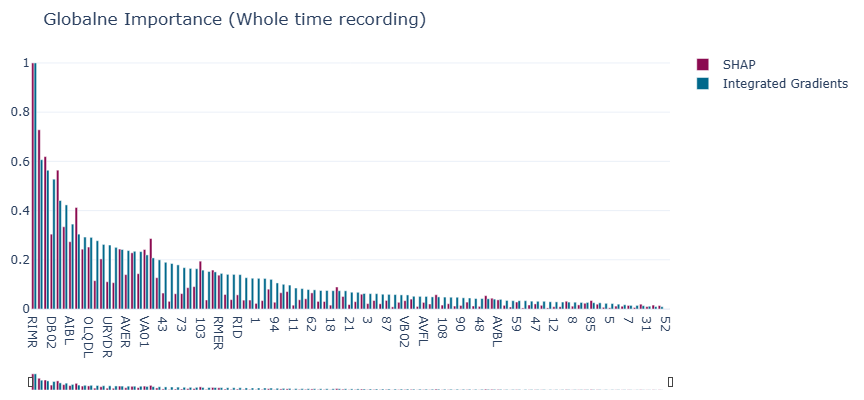
\includegraphics[width=0.95\textwidth]{plot_1.png} 
    \caption{Distribution of SHAP and IG values per neuron for a single recording (Worm I), illustrating the exponential decay in feature importance.}
    \label{fig:wykres2}
\end{figure}

To quantitatively validate that this
 sparse representation captures the true decision-making process
of the model rather than being an artifact of the explainer,
we conducted a Retain-And-Retrain (RAR) evaluation following the protocol introduced
by Rahman et al. (2022) \cite{rahman2022interpreting}. Strikingly, when restricting
the input space to only the top 10\% most salient neurons, the model maintained an accuracy of 95\% or higher. 

This computational sparsity aligns perfectly with fundamental principles
of systems neuroscience. As highlighted by Cunningham and Yu (2014) \cite{cunningham2014dimensionality},
neural population activity typically resides on a low-dimensional manifold governed by a small number of latent collective drivers,
rendering much of the high-dimensional single-neuron activity redundant. Furthermore, our findings corroborate the
observations made by Kato et al. (2015) \cite{kato2015global} in \textit{C. elegans}. Their research demonstrated
that although the activity of over 100 neurons can be recorded simultaneously,
just three principal components are sufficient to explain over 65\% of the variance,
implying that only a small, core subset of neurons actively drives global behavioral states.

The fact that BunDLe-Net preserves its full predictive power
 when restricted to this minimal neural subset confirms that the model's latent
representation successfully isolates the core computational manifold of the worm's nervous
system. Consequently, this extreme concentration of feature importance provides a
vital methodological foundation for our subsequent analyses. 
To accurately assess the stability and biological validity
of the model, the following sections will focus specifically on the highly salient
neural core using rank-aware and Top-$k$ metrics.



\subsubsection{Overall comparison}

In tables below the results of XAI methods are presented. Each table corresponds to one behavior. Note that neurons idetified as most importnat by Kato et al. are highlighted in the bold blue color. 

\newcommand{\kato}[1]{\textcolor{blue}{\textbf{#1}}}

\begin{table}[H]
    \centering
    \footnotesize % Zmniejszenie czcionki, aby 11 kolumn zmieściło się na stronie
    \renewcommand{\arraystretch}{1.2}
    \setlength{\tabcolsep}{3pt} % Zmniejszenie odstępów między kolumnami
    
    \begin{tabularx}{\textwidth}{@{} c *{10}{>{\centering\arraybackslash}X} @{}}
        \toprule
        & \multicolumn{2}{c}{\textbf{Worm 1}} 
        & \multicolumn{2}{c}{\textbf{Worm 2}} 
        & \multicolumn{2}{c}{\textbf{Worm 3}} 
        & \multicolumn{2}{c}{\textbf{Worm 4}} 
        & \multicolumn{2}{c}{\textbf{Worm 5}} \\
        \cmidrule(lr){2-3} \cmidrule(lr){4-5} \cmidrule(lr){6-7} \cmidrule(lr){8-9} \cmidrule(lr){10-11}
        \textbf{Place} 
        & \textbf{IG} & \textbf{SHAP} 
        & \textbf{IG} & \textbf{SHAP} 
        & \textbf{IG} & \textbf{SHAP} 
        & \textbf{IG} & \textbf{SHAP} 
        & \textbf{IG} & \textbf{SHAP} \\
        \midrule
        1 & OLQVL & OLQVL & AIBR & VB01 & \kato{RMED} & RMEV & \kato{RMED} & 53 & AIBR & \kato{RMED} \\
        2 & OLQDL & DB02 & OLQDL & OLQDL & RIMR & \kato{RMED} & DA01 & DA01 & AVER & RMEV \\
        3 & AIBR & \kato{RMED} & OLQVR & RMEV & AVER & RIMR & AS01 & OLQVL & \kato{RMED} & AIBR \\
        4 & OLQVR & OLQDL & RIMR & AIBR & RIVL & VB01 & SIBVL & AS01 & 24 & 24 \\
        5 & RIMR & AIBR & ASKR & 54 & 18 & AVER & OLQVL & SIBVL & 20 & AVER \\
        6 & RIML & AVEL & RIVR & 10 & 31 & AVBR & AIBR & RIVL & VA01 & 20 \\
        7 & AVEL & RIML & 66 & RIMR & AVEL & AIBR & 53 & RMER & 22 & RIMR \\
        8 & RIVR & OLQVR & 54 & RIFR & 128 & RIVL & SABVR & RIVR & 126 & 49 \\
        9 & 99 & RIMR & RMER & OLQVR & 125 & 26 & 59 & AVBR & ALA & 18 \\
        10 & AIBL & RIVR & 7 & RIVR & RMEV & RMER & RIVL & RIMR & AVFR & RIML \\
        \bottomrule
    \end{tabularx}
    \caption{Comparison of Top 10 rankings for \textbf{Dorsal turn} behavior}
    \label{tab:dorsal_turn_rankings}
\end{table}

\begin{table}[H]
    \centering
    \footnotesize 
    \renewcommand{\arraystretch}{1.2}
    \setlength{\tabcolsep}{3pt} 
    
    \begin{tabularx}{\textwidth}{@{} c *{10}{>{\centering\arraybackslash}X} @{}}
        \toprule
        & \multicolumn{2}{c}{\textbf{Worm 1}} 
        & \multicolumn{2}{c}{\textbf{Worm 2}} 
        & \multicolumn{2}{c}{\textbf{Worm 3}} 
        & \multicolumn{2}{c}{\textbf{Worm 4}} 
        & \multicolumn{2}{c}{\textbf{Worm 5}} \\
        \cmidrule(lr){2-3} \cmidrule(lr){4-5} \cmidrule(lr){6-7} \cmidrule(lr){8-9} \cmidrule(lr){10-11}
        \textbf{Place} 
        & \textbf{IG} & \textbf{SHAP} 
        & \textbf{IG} & \textbf{SHAP} 
        & \textbf{IG} & \textbf{SHAP} 
        & \textbf{IG} & \textbf{SHAP} 
        & \textbf{IG} & \textbf{SHAP} \\
        \midrule
        1 & DB02 & RIMR & DB01 & RIMR & VB02 & VB02 & 61 & RIML & 127 & 127 \\
        2 & RMED & RIML & RMER & DB01 & RMED & RMED & RMED & ASKL & \kato{RMEV} & VA01 \\
        3 & \kato{AVBR} & AIBR & SIBDR & AIBR & \kato{RMEV} & RIML & VB02 & RID & RMED & \kato{RMEV} \\
        4 & URYDR & RMED & RIVR & RIML & 82 & RIMR & SIBVL & AIBR & VA01 & RIMR \\
        5 & 43 & RIVR & AIBR & RMER & 83 & RIVL & RIS & RMED & 54 & RMED \\
        6 & 109 & AVEL & VB01 & RIVR & 76 & AIBL & 7 & 117 & \kato{AVBL} & AIBR \\
        7 & ASKL & OLQDL & 66 & 54 & RIVL & AIBR & URYDL & VB01 & 87 & 1 \\
        8 & RID & \kato{AVBR} & VB02 & RIFR & SIADL & 83 & ALA & RIVL & 15 & \kato{AVBL} \\
        9 & RIMR & AIBL & RMEL & VB02 & VB01 & \kato{RMEV} & ASKL & SIBVL & 129 & RIVL \\
        10 & DB01 & \kato{RMEV} & VB03 & VB01 & \kato{AVBR} & 82 & AVFL & RMEL & 120 & ASKR \\
        \bottomrule
    \end{tabularx}
    \caption{Comparison of Top 10 rankings for \textbf{Forward} behavior}
    \label{tab:forward_rankings}
\end{table}

\begin{table}[H]
    \centering
    \footnotesize 
    \renewcommand{\arraystretch}{1.2}
    \setlength{\tabcolsep}{3pt} 
    
    \begin{tabularx}{\textwidth}{@{} c *{10}{>{\centering\arraybackslash}X} @{}}
        \toprule
        & \multicolumn{2}{c}{\textbf{Worm 1}} 
        & \multicolumn{2}{c}{\textbf{Worm 2}} 
        & \multicolumn{2}{c}{\textbf{Worm 3}} 
        & \multicolumn{2}{c}{\textbf{Worm 4}} 
        & \multicolumn{2}{c}{\textbf{Worm 5}} \\
        \cmidrule(lr){2-3} \cmidrule(lr){4-5} \cmidrule(lr){6-7} \cmidrule(lr){8-9} \cmidrule(lr){10-11}
        \textbf{Place} 
        & \textbf{IG} & \textbf{SHAP} 
        & \textbf{IG} & \textbf{SHAP} 
        & \textbf{IG} & \textbf{SHAP} 
        & \textbf{IG} & \textbf{SHAP} 
        & \textbf{IG} & \textbf{SHAP} \\
        \midrule
        1 & \kato{RIMR} & \kato{AIBR} & RIVR & RIVR & RMEV & RMED & RIVL & RMED & VA01 & RMED \\
        2 & \kato{AIBR} & \kato{AVEL} & \kato{AIBR} & \kato{AIBR} & RIVL & RIVL & \kato{AIBL} & \kato{AIBR} & \kato{AIBR} & \kato{AVER} \\
        3 & RIVR & \kato{RIMR} & 106 & \kato{AVEL} & \kato{RIMR} & \kato{AVEL} & \kato{AIBR} & \kato{AIBL} & RMEV & \kato{RIML} \\
        4 & \kato{AIBL} & RMED & RIVL & 106 & VB01 & AVBR & RIGL & RIVL & VB02 & RMEV \\
        5 & \kato{RIML} & RIVR & ASKR & SIBDR & RMED & 105 & \kato{AVEL} & SIBVL & 128 & VA01 \\
        6 & DB02 & DB02 & \kato{AIBL} & \kato{RIML} & \kato{AIBL} & \kato{RIMR} & 51 & \kato{AVEL} & 15 & \kato{AVEL} \\
        7 & 109 & OLQVL & RID & \kato{RIMR} & \kato{AVER} & \kato{AVER} & ASKL & SABD & 127 & 127 \\
        8 & URYDR & \kato{AIBL} & ASKL & \kato{AVER} & AVBR & RMEV & SABVR & RIVR & 54 & \kato{AIBR} \\
        9 & OLQDL & OLQDL & \kato{RIMR} & ASKR & \kato{AIBR} & VB01 & RIGR & OLQDL & ASKR & ASKR \\
        10 & 73 & VA01 & 104 & RIVL & 18 & 32 & 59 & ALA & 119 & 128 \\
        \bottomrule
    \end{tabularx}
    \caption{Comparison of Top 10 rankings for\textbf{ Reverse-1} behavior}
    \label{tab:reverse_1_rankings}
\end{table}

\begin{table}[H]
    \centering
    \footnotesize 
    \renewcommand{\arraystretch}{1.2}
    \setlength{\tabcolsep}{3pt} 
    
    \begin{tabularx}{\textwidth}{@{} c *{10}{>{\centering\arraybackslash}X} @{}}
        \toprule
        & \multicolumn{2}{c}{\textbf{Worm 1}} 
        & \multicolumn{2}{c}{\textbf{Worm 2}} 
        & \multicolumn{2}{c}{\textbf{Worm 3}} 
        & \multicolumn{2}{c}{\textbf{Worm 4}} 
        & \multicolumn{2}{c}{\textbf{Worm 5}} \\
        \cmidrule(lr){2-3} \cmidrule(lr){4-5} \cmidrule(lr){6-7} \cmidrule(lr){8-9} \cmidrule(lr){10-11}
        \textbf{Place} 
        & \textbf{IG} & \textbf{SHAP} 
        & \textbf{IG} & \textbf{SHAP} 
        & \textbf{IG} & \textbf{SHAP} 
        & \textbf{IG} & \textbf{SHAP} 
        & \textbf{IG} & \textbf{SHAP} \\
        \midrule
        1 & RMED & \kato{AVEL} & \kato{AIBR} & RIVR & \kato{AIBR} & RIVL & \kato{AIBR} & \kato{RIML} & \kato{RIMR} & \kato{AVER} \\
        2 & \kato{AIBR} & RMED & \kato{AIBL} & \kato{AVEL} & \kato{AIBL} & \kato{AIBR} & \kato{AIBL} & \kato{AIBR} & \kato{AIBR} & \kato{AIBR} \\
        3 & \kato{RIMR} & RIVR & SIBDR & \kato{AIBR} & 89 & \kato{AVEL} & SIBVL & \kato{AIBL} & VB02 & \kato{RIMR} \\
        4 & DB02 & \kato{RIMR} & \kato{RIMR} & DB01 & RMED & VB01 & RMED & SIBVL & RMED & RMEV \\
        5 & \kato{AIBL} & \kato{AIBR} & VB03 & RIVL & VB01 & \kato{AVER} & ASKL & \kato{AVEL} & RMEV & \kato{AVEL} \\
        6 & 35 & AVBR & RIVR & \kato{RIMR} & 16 & \kato{AIBL} & \kato{RIML} & RMED & 127 & RMED \\
        7 & DB01 & RIVL & DB02 & \kato{RIML} & \kato{RIML} & RMED & 37 & RIVL & 50 & VA01 \\
        8 & 38 & OLQDL & ASKL & VB03 & \kato{AVER} & 105 & SABD & ASKL & 54 & VB02 \\
        9 & 109 & 35 & DB01 & SIBDR & RIVL & \kato{RIML} & SAAVR & AVBR & VA01 & AVBL \\
        10 & VB01 & VB01 & RID & 40 & 120 & \kato{RIMR} & AVBR & SAAVR & 120 & 87 \\
        \bottomrule
    \end{tabularx}
    \caption{Comparison of Top 10 rankings for \textbf{Reverse-2} behavior}
    \label{tab:reverse_2_rankings}
\end{table}

\begin{table}[H]
    \centering
    \footnotesize 
    \renewcommand{\arraystretch}{1.2}
    \setlength{\tabcolsep}{3pt} 
    
    \begin{tabularx}{\textwidth}{@{} c *{10}{>{\centering\arraybackslash}X} @{}}
        \toprule
        & \multicolumn{2}{c}{\textbf{Worm 1}} 
        & \multicolumn{2}{c}{\textbf{Worm 2}} 
        & \multicolumn{2}{c}{\textbf{Worm 3}} 
        & \multicolumn{2}{c}{\textbf{Worm 4}} 
        & \multicolumn{2}{c}{\textbf{Worm 5}} \\
        \cmidrule(lr){2-3} \cmidrule(lr){4-5} \cmidrule(lr){6-7} \cmidrule(lr){8-9} \cmidrule(lr){10-11}
        \textbf{Place} 
        & \textbf{IG} & \textbf{SHAP} 
        & \textbf{IG} & \textbf{SHAP} 
        & \textbf{IG} & \textbf{SHAP} 
        & \textbf{IG} & \textbf{SHAP} 
        & \textbf{IG} & \textbf{SHAP} \\
        \midrule
        1 & \kato{RIMR} & \kato{RIMR} & \kato{RIMR} & \kato{RIMR} & \kato{RIML} & \kato{AIBR} & \kato{AIBL} & \kato{AIBR} & \kato{RIML} & VA01 \\
        2 & \kato{RIML} & \kato{RIML} & \kato{AIBR} & \kato{RIML} & \kato{AVEL} & RMED & \kato{AIBR} & RMED & VA01 & \kato{AIBR} \\
        3 & \kato{AVEL} & \kato{AVEL} & \kato{RIML} & \kato{AIBR} & \kato{AVER} & \kato{AIBL} & DA01 & \kato{AIBL} & \kato{RIMR} & \kato{RIML} \\
        4 & \kato{AIBR} & RMED & \kato{AVEL} & RIVR & RIVL & \kato{AVER} & AS01 & DA01 & \kato{AIBR} & RMED \\
        5 & \kato{AVER} & DB01 & RIVR & \kato{AVER} & 126 & \kato{RIML} & ASKL & \kato{RIMR} & \kato{AVEL} & RMEV \\
        6 & \kato{AIBL} & VA01 & \kato{AIBL} & DB01 & 31 & 105 & \kato{RIMR} & AS01 & \kato{AVER} & AVBL \\
        7 & VA01 & 103 & RIGL & \kato{AVEL} & \kato{AIBR} & AVBR & AVFR & AVBL & ALA & \kato{AIBL} \\
        8 & OLQDL & \kato{AIBR} & 40 & SIBDR & 89 & \kato{RIMR} & 28 & OLQVL & 126 & \kato{RIMR} \\
        9 & DB02 & DB02 & 108 & ASKR & 118 & RIVL & \kato{AVEL} & RIVL & 1 & \kato{AVER} \\
        10 & 109 & \kato{AIBL} & ASKR & VB02 & 128 & ASKR & OLQVL & RMER & 128 & \kato{AVEL} \\
        \bottomrule
    \end{tabularx}
    \caption{Comparison of Top 10 rankings for \textbf{Sustained reversal} behavior}
    \label{tab:sustained_reversal_rankings}
\end{table}

\begin{table}[H]
    \centering
    \footnotesize 
    \renewcommand{\arraystretch}{1.2}
    \setlength{\tabcolsep}{3pt} 
    
    \begin{tabularx}{\textwidth}{@{} c *{10}{>{\centering\arraybackslash}X} @{}}
        \toprule
        & \multicolumn{2}{c}{\textbf{Worm 1}} 
        & \multicolumn{2}{c}{\textbf{Worm 2}} 
        & \multicolumn{2}{c}{\textbf{Worm 3}} 
        & \multicolumn{2}{c}{\textbf{Worm 4}} 
        & \multicolumn{2}{c}{\textbf{Worm 5}} \\
        \cmidrule(lr){2-3} \cmidrule(lr){4-5} \cmidrule(lr){6-7} \cmidrule(lr){8-9} \cmidrule(lr){10-11}
        \textbf{Place} 
        & \textbf{IG} & \textbf{SHAP} 
        & \textbf{IG} & \textbf{SHAP} 
        & \textbf{IG} & \textbf{SHAP} 
        & \textbf{IG} & \textbf{SHAP} 
        & \textbf{IG} & \textbf{SHAP} \\
        \midrule
        1 & RMED & RMED & SIBDR & RIMR & RMED & \kato{AIBR} & RMED & \kato{AIBR} & AVBL & RMEV \\
        2 & DB02 & RIMR & RMED & RIML & 105 & RMED & AVFR & RMED & 127 & \kato{AIBR} \\
        3 & AVBR & RMEV & DB01 & \kato{AIBR} & AVBR & \kato{AIBL} & SIBVL & \kato{AIBL} & RMEV & AVBL \\
        4 & RMEV & AVEL & \kato{AIBL} & RIVR & RMEV & AVBR & RIS & DA01 & 87 & VA01 \\
        5 & VB01 & RIML & RMEL & AVEL & 67 & 105 & AVBL & AS01 & ASKR & RIML \\
        6 & DB01 & \kato{AIBL} & 66 & AVER & VB02 & AVER & \kato{AIBL} & RIMR & 125 & \kato{AIBL} \\
        7 & RMER & DB02 & VB03 & VB01 & VB01 & RMER & RMEL & AVBL & VB02 & RIMR \\
        8 & URYDL & AVBR & VB01 & VB02 & RIS & ASKR & VB01 & RMER & ALA & AVEL \\
        9 & 93 & VA01 & RIVR & RMED & RMER & 83 & RMER & SIBVL & 120 & RMED \\
        10 & RIVR & DB01 & DB02 & ASKL & 82 & 67 & \kato{AIBR} & RIS & 1 & 127 \\
        \bottomrule
    \end{tabularx}
    \caption{Comparison of Top 10 rankings for \textbf{Slowing} behavior}
    \label{tab:slowing_rankings}
\end{table}

\begin{table}[H]
    \centering
    \footnotesize 
    \renewcommand{\arraystretch}{1.2}
    \setlength{\tabcolsep}{3pt} 
    
    \begin{tabularx}{\textwidth}{@{} c *{10}{>{\centering\arraybackslash}X} @{}}
        \toprule
        & \multicolumn{2}{c}{\textbf{Worm 1}} 
        & \multicolumn{2}{c}{\textbf{Worm 2}} 
        & \multicolumn{2}{c}{\textbf{Worm 3}} 
        & \multicolumn{2}{c}{\textbf{Worm 4}} 
        & \multicolumn{2}{c}{\textbf{Worm 5}} \\
        \cmidrule(lr){2-3} \cmidrule(lr){4-5} \cmidrule(lr){6-7} \cmidrule(lr){8-9} \cmidrule(lr){10-11}
        \textbf{Place} 
        & \textbf{IG} & \textbf{SHAP} 
        & \textbf{IG} & \textbf{SHAP} 
        & \textbf{IG} & \textbf{SHAP} 
        & \textbf{IG} & \textbf{SHAP} 
        & \textbf{IG} & \textbf{SHAP} \\
        \midrule
        1 & \kato{RIVL} & \kato{RIVR} & SIBDR & \kato{RIVR} & \kato{RIVL} & \kato{RIVL} & AIBR & \kato{RIVL} & \kato{RIVL} & \kato{RIVL} \\
        2 & AVEL & \kato{RIVL} & AIBR & \kato{RIVL} & AIBR & RMED & \kato{RIVL} & RIML & VA01 & 127 \\
        3 & RIMR & AVEL & AVEL & RIML & AVER & AIBR & AIBL & ASKL & 26 & VA01 \\
        4 & \kato{RIVR} & RMEV & ASKL & SIBDR & AIBL & 54 & ASKL & RMED & RIMR & RMED \\
        5 & OLQDL & RMED & RIML & DB01 & AVEL & AVER & RIML & AVEL & AIBR & RIMR \\
        6 & OLQVL & OLQVL & RIMR & 40 & RIML & 29 & AVBR & AVBR & 127 & 26 \\
        7 & AIBR & RIMR & AIBL & AIBR & 54 & VB02 & 28 & AIBR & 15 & RMEV \\
        8 & AIBL & OLQVR & \kato{RIVR} & OLQDL & 29 & AVEL & SABD & \kato{RIVR} & 54 & AIBR \\
        9 & 93 & OLQDL & OLQDR & RIMR & ASKR & 32 & AVEL & SAAVL & ALA & AVER \\
        10 & RMEV & VA01 & VB03 & AVEL & RMEV & AIBL & 37 & 28 & 28 & RIML \\
        \bottomrule
    \end{tabularx}
    \caption{Comparison of Top 10 rankings for \textbf{Ventral turn} behavior}
    \label{tab:ventral_turn_rankings}
\end{table}

As demonstrated in the tables above, the reference neurons identified by Kato et al. (2015) \cite{kato2015global} frequently emerge within the highest-ranking positions across multiple behavioral states and individual worms. However, in several instances, key reference neurons fail to reach the top ranks. Furthermore, the feature importance profiles exhibit noticeable variability both between individual worms and across different feature attribution methods—specifically, SHAP \cite{lundberg2017unified} and Integrated Gradients \cite{sundararajan2017axiomatic}.

Moreover, the results indicate that neurons idefntifies as crucial for one specific behavior also frequently appear as highly important in others, even when they were not explicitly highlighted by Kato et al. for that particular movement. This outcome demonstrates that neurons do not operate in an isolated manner; rather, they are integrated into a shared population dynamics framework and perform coordinated roles in driving state transitions \cite{vyas2020computation}. Consequently, neuron families such as RMED, AVE, RIM, or AVB consistently recur across all behavioral rankings.

Additionally, the feature rankings reveal not only known reference neurons but also unidentified neurons (e.g., neurons 127 and 61 in Forward locomotion), which occasionally occupy the top rank. This indicates that their underlying neural activity provides a crucial predictive signal for the model during these behavioral states.

The recurrent presence of these biological ground-truth neurons suggests
that BunDLe-Net's latent representations successfully capture the true 
underlying neural dynamics of \textit{C. elegans} locomotion, rather than
relying on spurious correlations or noise. Nevertheless, as highlighted
in interpretability literature \cite{lipton2018mythos}, a mere visual inspection of top-10 attribution rankings
 is insufficient to establish definitive conclusions regarding model alignment and trustworthiness \cite{mathis2026joint}.
Because these qualitative results cannot fully validate the model's robustness,
a rigorous quantitative correlation analysis was incorporated to evaluate the hypothesis.

As mentioned in the \textbf{Diminishing saliency of the neurons} sub-section, this type of data
frequently encounter the challenge of tail noise dominance. Consistent 
with the low-dimensional manifold hypothesis in systems neuroscience \cite{cunningham2014dimensionality}
and feature pruning studies \cite{rahman2022interpreting}, only a compact subset of leading neurons
(approximately 5--10\%) drives the model's behavioral predictions,
while the remaining majority contributes negligible signal or background noise.
Under such heavy tail noise, conventional metrics like the global Spearman rank correlation
yield distorted and untrustworthy results, as random rank permutations among near-zero attributions
disproportionately dilute the correlation of genuine leading drivers \cite{webber2010similarity}.
To mitigate this issue and isolate the biologically meaningful signal, we incorporated two top-weighted
similarity metrics established in information retrieval and interpretability literature: the Top-$k$ Jaccard Similarity
and the Rank-Biased Overlap (RBO) coefficient \cite{webber2010similarity}.



\subsubsection{Correlation between worms}

As stated by Mathis and Mathis (2026) \cite{mathis2026joint}, joint-modeling model should perform similar across different subjects so we are assured that it generalized the behaviour of the brain, To test that the inter-worm correlation was calculated. The results for 10 unique worm pairs were shown in the table 9 below. The `Mean $\rho \pm$ SD' columns display the average correlation coefficient and standard deviation. The `Sig. Pairs' columns indicate the number of pairs that achieved statistical significance ($p < 0.05$)

\begin{table}[H]
    \centering
    \renewcommand{\arraystretch}{1.3} 
    \begin{tabular}{l c c}
        \toprule
        \textbf{Behavioral State} & \textbf{Mean RBO ($p=0.9$) $\pm$ SD} & \textbf{Mean Top-10 Jaccard $\pm$ SD} \\
        \midrule
        \textbf{Global (All states)} & 0.397 $\pm$ 0.118 & 0.339 $\pm$ 0.091 \\
        \textbf{Dorsal Turn}         & 0.253 $\pm$ 0.115 & 0.211 $\pm$ 0.086 \\
        \textbf{Forward}             & 0.331 $\pm$ 0.110 & 0.240 $\pm$ 0.086 \\
        \textbf{Reverse-1}           & 0.364 $\pm$ 0.084 & 0.254 $\pm$ 0.074 \\
        \textbf{Reverse-2}           & 0.368 $\pm$ 0.069 & 0.304 $\pm$ 0.085 \\
        \textbf{Sustained Reversal}  & 0.415 $\pm$ 0.126 & 0.333 $\pm$ 0.104 \\
        \textbf{Slowing}             & 0.376 $\pm$ 0.093 & 0.259 $\pm$ 0.111 \\
        \textbf{Ventral Turn}        & 0.406 $\pm$ 0.083 & 0.260 $\pm$ 0.055 \\
        \textbf{No state}            & 0.131 $\pm$ 0.104 & 0.075 $\pm$ 0.078 \\
        \bottomrule
    \end{tabular}
    \caption{Summary of inter-worm attribution consistency across all defined behavioral states (\textbf{SHAP})}
    \label{tab:inter_worm_summary_I}
\end{table}

\begin{table}[H]
    \centering
    \renewcommand{\arraystretch}{1.3} 
    \begin{tabular}{l c c}
        \toprule
        \textbf{Behavioral State} & \textbf{Mean RBO ($p=0.9$) $\pm$ SD} & \textbf{Mean Top-10 Jaccard $\pm$ SD} \\
        \midrule
        \textbf{Global (All states)} & 0.350 $\pm$ 0.106 & 0.240 $\pm$ 0.086 \\
        \textbf{Dorsal Turn}         & 0.234 $\pm$ 0.114 & 0.110 $\pm$ 0.079 \\
        \textbf{Forward}             & 0.174 $\pm$ 0.076 & 0.077 $\pm$ 0.038 \\
        \textbf{Reverse-1}           & 0.255 $\pm$ 0.071 & 0.154 $\pm$ 0.074 \\
        \textbf{Reverse-2}           & 0.395 $\pm$ 0.081 & 0.187 $\pm$ 0.069 \\
        \textbf{Sustained Reversal}  & 0.389 $\pm$ 0.142 & 0.265 $\pm$ 0.099 \\
        \textbf{Slowing}             & 0.301 $\pm$ 0.132 & 0.167 $\pm$ 0.114 \\
        \textbf{Ventral Turn}        & 0.380 $\pm$ 0.097 & 0.247 $\pm$ 0.080 \\
        \textbf{No state}            & 0.134 $\pm$ 0.064 & 0.108 $\pm$ 0.056 \\
        \bottomrule
    \end{tabular}
    \caption{Summary of inter-worm attribution consistency across all defined behavioral states (\textbf{Integrated gradients})}
    \label{tab:inter_worm_summary_II}
\end{table}


\begin{figure}[H]
    \centering
    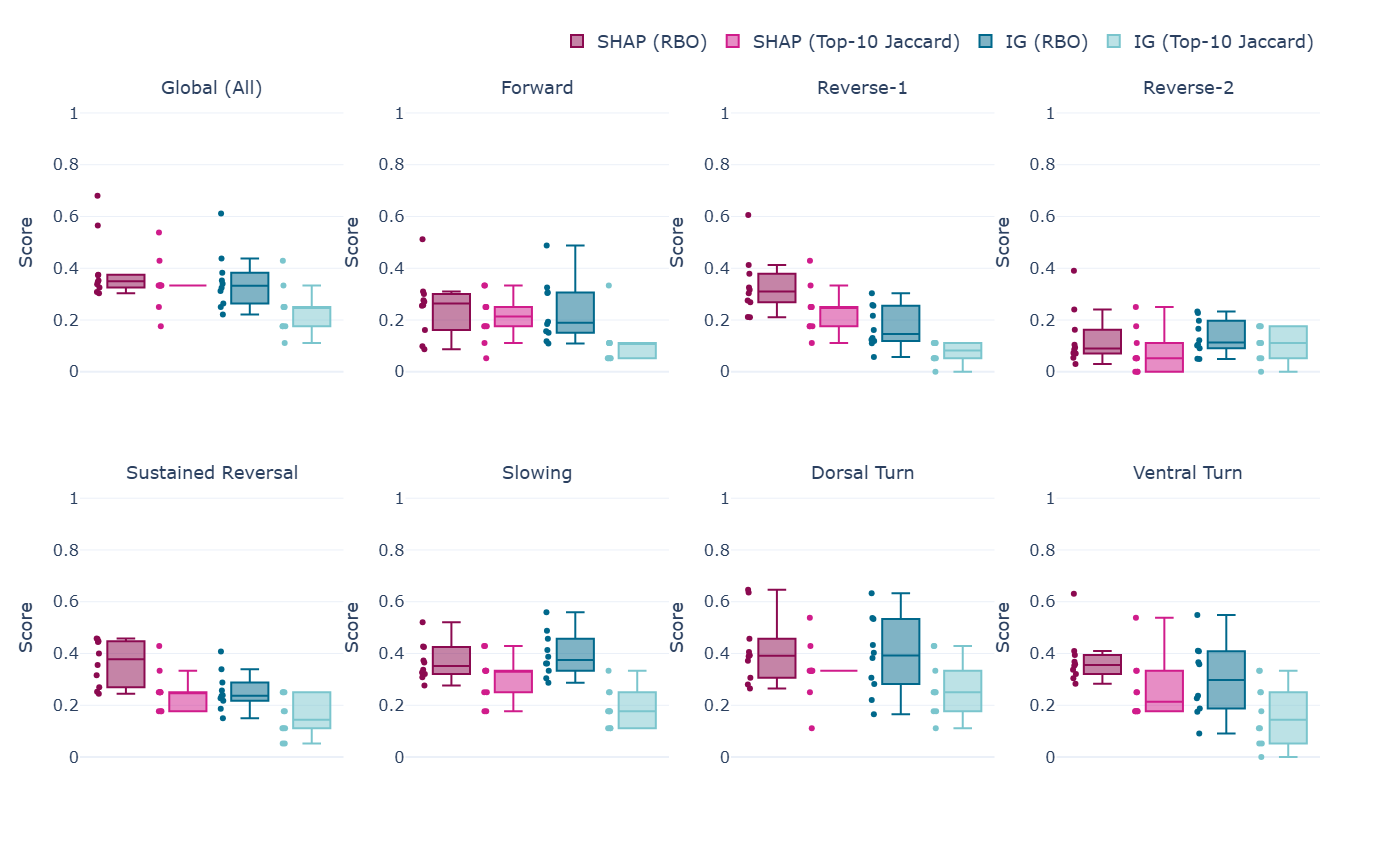
\includegraphics[width=0.95\textwidth]{boxplots.png} 
    \caption{Compassion of SHAP and IG results correlation between worms per each behaviour}
    \label{fig:wykres1}
\end{figure}

At first glance, the results might seem unsatisfying,
 as the absolute consistency values across all comparisons are relatively low.
However, in the context of biological data from \textit{C. elegans}, we view these results as highly realistic and valuable.

Firstly, the coefficients across both XAI methods drop significantly
for the "No state" category. During periods without a defined behavioral state,
there should not be any specific command neurons taking the lead in the worm's brain \cite{kato2015global}.
This means that across different worms, we should not expect to see any recurring ranking patterns.
This hypothesis perfectly aligns with our findings, the consistency for the "No state" category is virtually non-existent.

Compared to the "No state" baseline,
defined behavioral states exhibit up to four times stronger consistency.
This is a highly positive outcome, suggesting that BunDLe-Net's predictions are grounded in consistent
biological trends rather than the idiosyncratic noise of individual worms brains. Moreover, results occurring mostly
 in the 0.30--0.40 range are well-supported by the concept of neural degeneracy \cite{edelman2001degeneracy}.
A Top-10 Jaccard value in this range indicates that, on average, 3 to 4 neurons in the top ranking are shared across worms,
while the rest vary. This clearly demonstrates that while executing the same behavior, different worms rely on the same 3 to 4 core command neurons,
alongside different subsets of auxiliary neurons. This perfectly illustrates neural degeneracy, empirical evidence for which in \textit{Caenorhabditis elegans}
is reported by Trojanowski et al. (2014) \cite{trojanowski2014neural}.

Lastly, these results provide insight not only into BunDLe-Net's trustworthiness
but also into the performance of the chosen XAI methods. 
SHAP values have proven to be higher and significantly more stable than Integrated Gradients (IG) across almost all
behavioral states. For example, during the Forward behavior, the IG Jaccard score drops to as low as 0.077, which is practically at the level of statistical noise.
This demonstrates that SHAP performs much better in filtering out biological noise to identify true predictive features.




\subsubsection{Correlation between behaviours}

In their whole-brain imaging study, Kato et al. (2015) \cite{kato2015global} demonstrated
that the primary mode of neural variance (PC1) separates forward and backward locomotion.
Consequently, we hypothesize that feature attribution profiles between forward and backward
states will exhibit lower correlations, whereas states belonging to the same functional
family, such as Reverse-1, Reverse-2, and Sustained Reversal, will display strong positive correlations.
Nevertheless, based on our prior observations, some degree of
correlation is expected across behaviors, reflecting the continuous nature of low-dimensional neural manifolds. 

Because the cross-behavioral correlation patterns remain highly consistent
across individual worms, this subsection focuses on Worm 0 as a representative case. In the Table 10 and 11,
the cross-behaviour correlation was shown. 




\printbibliography

\end{document}
